\documentclass[journal,10pt,onecolumn,compsoc]{IEEEtran} \usepackage[margin=1.0in]{geometry} \usepackage{pdfpages} 

%\usepackage{color}
\usepackage{geometry}
\usepackage{graphicx}
\usepackage{amsthm}
\usepackage{amssymb}
\usepackage{amsmath}
\usepackage{float}
\usepackage{balance}
\usepackage{enumitem}
\usepackage{pstricks, pst-node}
\usepackage{hyperref}
\usepackage{url}

\hypersetup{
  colorlinks = true,
  urlcolor = cyan,
  pdfkeywords = {CS461``Senior Software Engr Project''Design Document},
  pdftitle = {CS 461 Progress Update },
  pdfsubject = {CS 461 Progress Update},
  pdfpagemode = UseNone
}

\begin{document}
\begin{center}
  
  \textbf{}

  \vspace{4cm}
  \Huge{}
  \textbf {Progress Report}
  \vspace{1.5cm}

 
  \LARGE
  CS461 - Senior Software Engr Project\\
  \vspace{0.25cm}
  Group 36: Data Interactive Visualization Application(DIVA)\\
  Instructor: D. Kevin McGrath \\
  Instructor: Kirsten Winters \\
  \vspace{0.25cm}
  Winter 2019 \\
  \vspace{1.5cm}
  
  \large{Bhavya Parikh, Davian Lukman, Eli Laudi, Matthew L. Jansen, and Ryan Sisco}\\
  \date{Feburary 25th, 2019}
  \vfill
  Feburary 25th, 2019\\
  \vspace{1cm}
  \vspace*{\fill}
   \begin{abstract}
       \noindent This purpose of this document is to examine and summarize the development of the Data Interactive Visualization Application (DIVA). Furthermore, this document will discuss the purpose and goals of our project, summarize the activities undergone in the past winter academic term, and finally define the current state of the project. 
   \end{abstract}
    \normalsize 
  \end{center}
\newpage
{\hypersetup{linkcolor=black}
\tableofcontents
}
\newpage

\section{Purpose and Goals}
\subsection{Purpose}
The purpose of our project is to develop an application that can absorb data stored in a comma-separated value file, or CSV file, and render the information into a 3D environment. Furthermore, this application will possess the ability to export these 3D environments into several file formats, including pictures, animations, and movie files. The DIVA web application will serve to the stakeholder as a tool to improve the overall understanding of large data sets, and more specifically understand the data's significance to a context provided by the stakeholder. The stakeholder can use this increased understanding of the data to present a large data set to a non-technical audience and effectively communicate the significance of the data while avoiding loss of understanding by the audience. 
\subsection{Goals}
The development team's goals for this term were to explore the different technologies that our project could integrate in order to fulfill the requirements provided by the stakeholder. Furthermore, another goal for this academic term was to build the documentation to properly outline the functionalities of the DIVA web application. Moving forward, our goals for the upcoming academic term include giving our stakeholder the opportunity to test our application by the end of the term. To accomplish this, the development team will work in conjunction with the stakeholder to create and execute sprint goals to ensure timely completion. 

\section{Weekly Summaries}
\subsection{Week 1}
    \subsubsection{Activities}
    This week, we made a Balsamiq design model of our project and send it to our client, so that we can receive feedback on how our team's perspective of the project differs from his. In addition, our group created 3 teams in order to divide the amount of work involved with implementing this project. Future plans include working in our respective teams on the tasks assigned, and meeting twice a week to discuss any difficulties encountered along the way. Currently, our plan is to meet every Tuesday to discuss problems related to inter-group interfacing, and meeting offline every Sunday to discuss general items. Furthermore, we emailed our client and stated that we are ready to proceed with development.  Lastly, our group created a design contract to define how each group will communicate with each other. 
    \subsubsection{Problems and Solutions}
    We are still having difficulties in setting up a meeting time with our client, as our client is very busy. Between our entire group, it is hard to find a specific time slot that works with everyone, however at the worst case scenario, we can meet over the weekend if our client approves. 
    
\subsection{Week 2}
    \subsubsection{Activities}
    This week, we have sent our client an email to engage in face-to-face communication, in order to get more feedback on our paper prototype, which was created last week. The client responded back with three questions about floating menu, changing axis, and samples of visualization. Based off of this information, our group was able to fix our UI prototype based on the client's feedback. From here, each member of the group was assigned a spot into any of the four available teams: UI, CSV parsing, 3D visualization, and exporting (we added one from last week). At this point, we decided that prioritizing the link between the UI and 3D visualization pages were essential, so 2 people were assigned to each of these teams, while the remaining team member was assigned to CSV parsing and exporting. We also made contact with our new TA, invited him to our GitHub and made set a time for weekly meetings.
    \subsubsection{Problems and Solutions}
    We do not have any problems as of right now because we will be using this week to establish contact with either the TA or client. We also fixed the prototype problem based on feedback from our client. We are still faced with the issue of not having good communication with our client, so we also planned to have a face-to-face meeting with the client at 23rd. Finally, in order to solve confusions about the visualization libraries needed for this project, the 3D visualization group planned to see Professor Bailey to ask further info about WebGL and access to CGEL lab.
    
\subsection{Week 3}
    \subsubsection{Activities}
    This week, we were able to finish our draft of the poster with help from TA. Our prototype was also approved by our client. Additionally, the client agreed to have a face-to-face meeting on Google Hangouts sometime in the near future. We are finally at a good starting point to begin implementing our application.
    \subsubsection{Problems and Solutions}
    The plan that we have in mind is to work on implementing our application soon, and begin our elevator pitch on Sunday. We will have a basic web layout after working over the weekend. Additionally, we will be meeting with our TA on Tuesday to ask for feedback on the UI. We also plan on using the elevator pitch in our meeting with the client on Wednesday, as well as presenting the UI during the meeting.
    
\subsection{Week 4}
    \subsubsection{Activities}
    This week, we were able to make progress in developing our web app by creating blank templates in localhost. By attending a group in-class meeting, we also learned of 10 takeaways that we should/shouldn't do at Expo. In addition, each team worked on developing their own section of code for the web application. 
    \subsubsection{Problems and Solutions}
    We tried to make our first face-to-face contact with our client, but for some reason, our client did not receive an email invitation for the Google Hangout. We tried to contact our client again to reschedule the meeting, however we did not get a response.
    Although our teams were able to make some progress this week, we did not get as much done as we would have liked, due to each team member having their own midterms this week. We aspire to get more done in the following week.
    
\subsection{Week 5}
    \subsubsection{Activities}
    We made significant progress this week. The 3DV team was able to make the rotate, pan, and zoom features for 3D visualization, which is the most important part for alpha release. The UI team managed to make some of the functionalities, along with working buttons. In the future, we plan to work on the thematic elements of the web-page, as well as integrating the front end with the back end.
    \subsubsection{Problems and Solutions}
    Our team was introduced to React for the first time (all except for one individual, who has quite a bit of experience in using the React engine). This caused us to slow down in implementation, as we had to learn a new environment. 
 
\subsection{Week 6}
    \subsubsection{Activities}
    This week, the  3D Visualization team made changes to 3D axes - we want the axes to look thicker, so we needed to make a new axes from scratch instead of using a built in functionality. Apart from that, CSV parsing made a lot of progress - the member in charge of this team finished a function which can correctly parse a data file with over 10000 entries. The UI team also made significant changes, which includes adding a header bar with a collapsible menu. Overall, we are ready to combine our results in order to take the input from CSV files, and visualize it soon.
    \subsubsection{Problems and Solutions}
    One problem that the CSV Parsing team encountered is that some values can contain commas themselves, although they aren't supposed to be separated; For example, IP address, type, etc. We also have had difficulties in combining the UI, rendering and CSV parser because we did not meet this week due to midterms. To counteract the CSV Parsing errors, we plan on just skipping rows that have a  more-than-expected amount of commas. Then, we will make a log in the bottom of the web-page that says a certain value was skipped due to inappropriate formatting. 
    
\subsection{Week 7}
    \subsubsection{Activities}
    This week we went to demonstrate our alpha release to the TA. We showed what we have so far, and we were able to obtain positive feedback from the TA. However, our alpha release does not represent the combination of CSV parser, rendering, and UI. We wanted to make this possible before sending alpha release to the client.
    \subsubsection{Problems and Solutions}
    Upon finished TA meeting, we asked who will be grading our project. The TA mentioned that the client will give us a grade. We have trouble handling this situation because our relationship with the client right now is not good. We were able to contact the client to hold a video call, but the client missed out and we did not get any reply from that time. This weekend, we will continue to work on combining and at least have the scatter plot ready to be sent to the client as alpha release. This will also be a new starting communication between us and the client.
 
 \subsection{Week 8}
    \subsubsection{Activities}
    This week, our group was able to get together and merge the UI teams' work with the CSV team. Doing this, we were able to get our web application to upload CSV files using a file explorer, and then afterwards fill in drop-down menus dynamically using this data. In addition, after the user uploads a file, it displays the filename so that the user knows which file they are using from their directory.
    \subsubsection{Problems and Solutions}
    During one of our meetings, the CSV and 3D Visualization team members noticed that their original contract for data interaction would not allow for complete data visualization. Although this is unfortunate, both of those teams began working out a plan to get around this obstacle, so that data can be efficiently drawn from the CSV file, and shipped to the 3D Visualization team. One idea was to convert the data points to coordinates before it is even sent to the 3DV team, however we are still exploring other options as well. 

    \subsection{Week 9}
    \subsubsection{Activities}
    This week, the 3D Visualization and CSV teams worked out a new contact in order to correctly plot the data into a 3D environment. These changes included adding meta-data, such as the amount of data and minimums/maximums in the data, into the JSON object. After this, the 3D Visualization and CSV teams' branches merged, so now we are able to actually plot data from a CSV file. This is a significant step towards our beta release. 
    \subsubsection{Problems and Solutions}
    We didn't run into many problems this week, the process of adding data to the CSV/3DV contact didn't add to much complexity. However, our group is a little more stressed about contacting our client. It's been a while since we had any contact with him, but we do not want to come to him without at least a beta-level release ready to test. 

    \subsection{Week 10}
    \subsubsection{Activities}
    This week, because the 3D Visualization and CSV team were able to complete their link last week, the exporting team was able to begin working with the canvas element produced by the 3D Visualization team. With this canvas element, the exporting team was able to download it to the user's web browser as a \emph{jpeg} image. With this done, we were able to merge the CSV/3DV/export team changes, along with an updated UI, into our final development branch. Using this branch, we were able to host this application using GitHub, and send it to our client as our beta release. We sent \href{https://ryansisco.github.io/DIVA/}{this link} to our client, along with an email detailing our progress, and our future steps. Our client responded promptly, he was very happy with our progress and understood that we were busy with school and life and couldn't get in contact with him sooner. He wants us to plan a call sometime in the next week or two. 
    \subsubsection{Problems and Solutions}
    We were able to get a lot done in the past two weeks, we did not run into any issues, however we are thinking of how we are going to overstep certain obstacles in the future. For example, we need to look further into downloading the canvas elements in \emph{GIF} and \emph{MP4} formats as well. To do this, we might incorporate auto-rotating views on the data while it is being rendered into the animation/movie. 
    
 \section{Current Status of Project}
 \subsection{Summary}
 In summary, we have developed each sector of our project to an alpha-release level. We aspire to soon combine each of these sectors together seamlessly, such that testing application-level data can be performed, such as testing different variable types within a given CSV file. 
 
 \subsection{Current Flow of Data}
 This subsection will define the current flow of data within our application.\newline
 \newline
 The DIVA web application first gives a blank screen, which gives the user the option to open up a menu, in the form of a pop-up modal. After doing this, the user will be presented with a variety of options, all of which are unavailable until the user uploads a CSV file using the \emph{Upload File} button. 
    
     \begin{figure}[H]
        \centering
        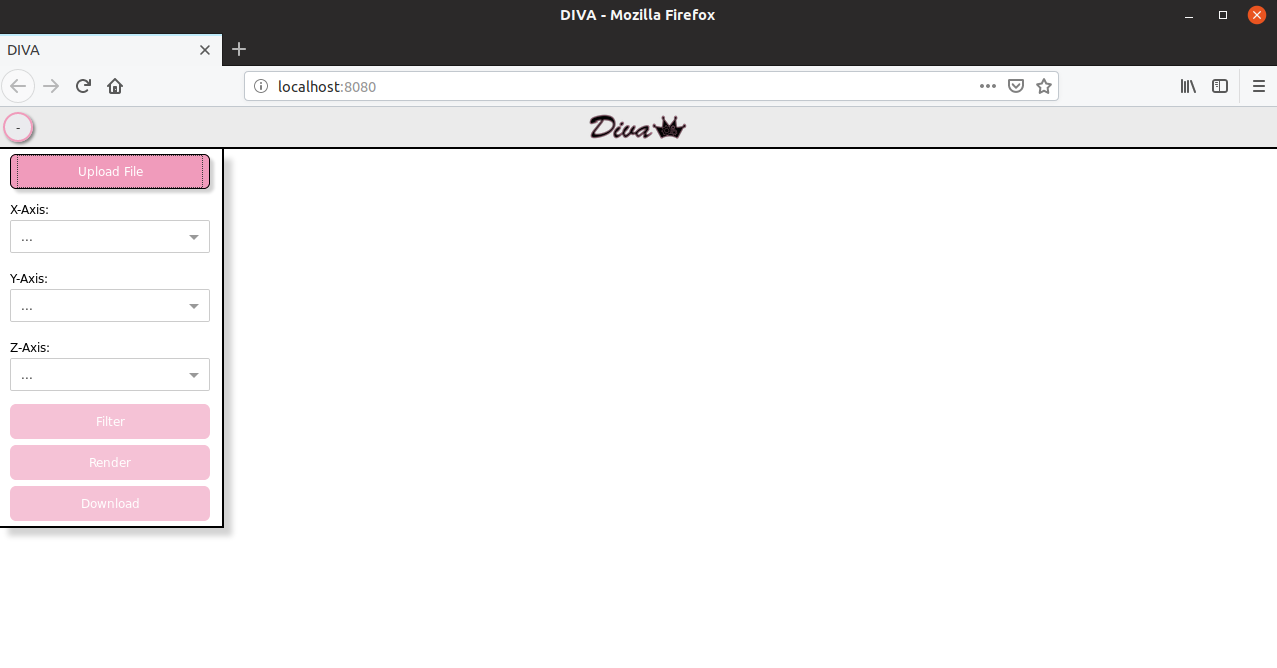
\includegraphics[width=\linewidth]{menu1.png}
        \caption{Initial menu given upon first opening up the pop-up menu}
    \end{figure}
 
 \newpage
 After selecting the \emph{Upload File} button, and selecting a CSV file, the remaining drop-down menus will be filled out with the titles given from the CSV file, as seen below.

     \begin{figure}[H]
        \centering
        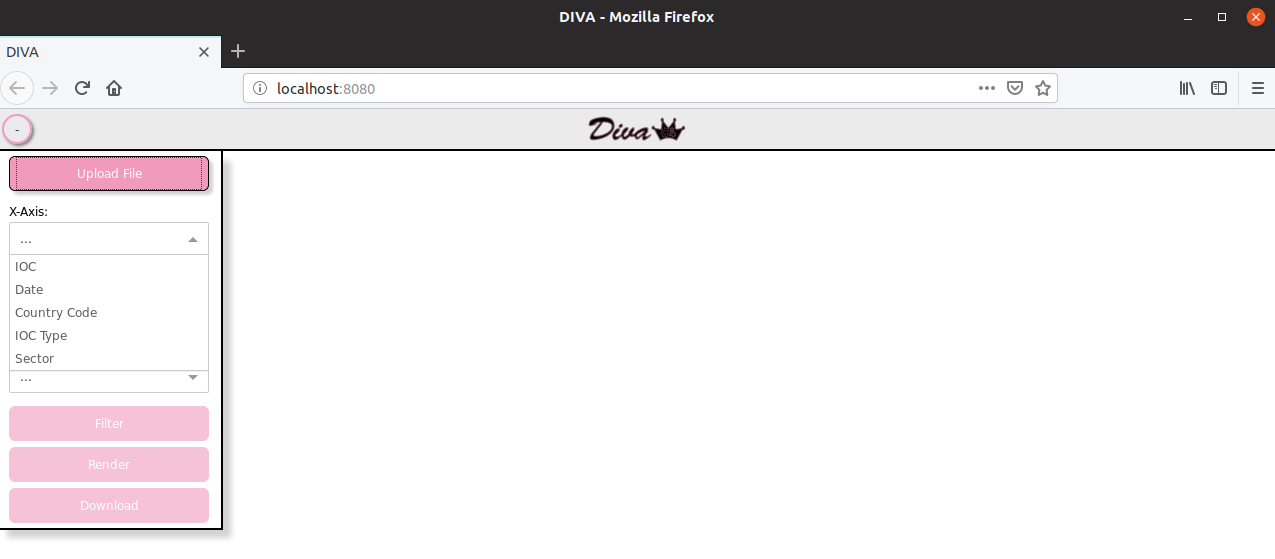
\includegraphics[width=\linewidth]{menu2.png}
        \caption{Example of drop-down menus opening up after the CSV file is uploaded}
    \end{figure}
 
 Once the drop-down menus are filled out with exclusively different options (such that no two axis have the same category), the remaining three buttons below the drop-down menus will become available to the user, as seen below. 

     \begin{figure}[H]
        \centering
        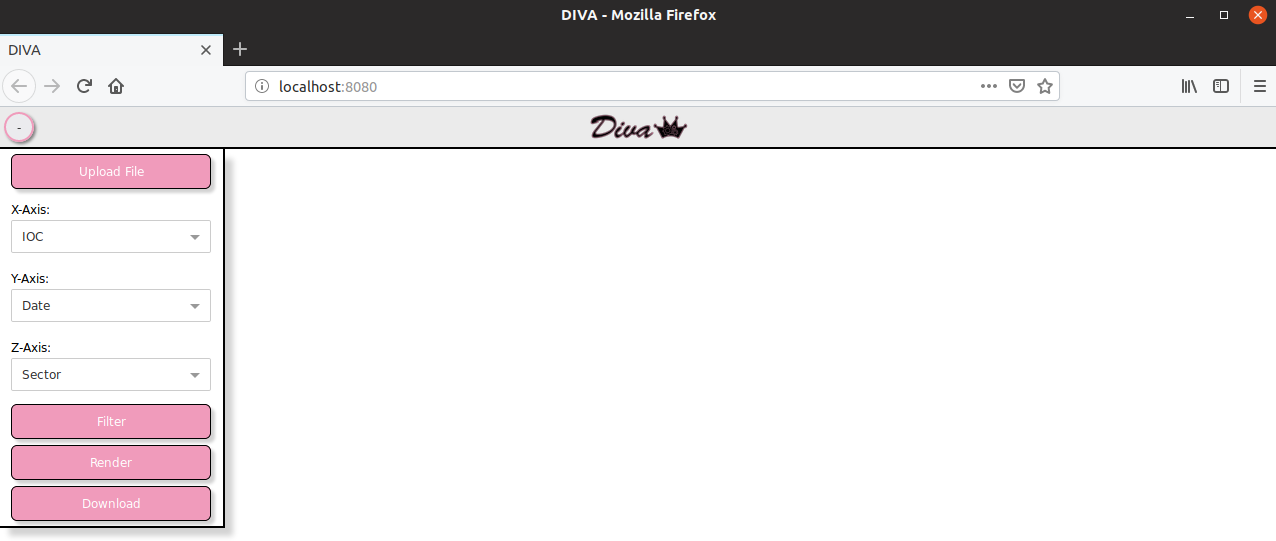
\includegraphics[width=\linewidth]{menu3.png}
        \caption{Example of the buttons in the lower part of the menu opening up after selecting categories}
    \end{figure}

Currently, our work effort entails bringing this UI together with visualizing the data in a 3D environment. Although the link between this UI and the graphics interface is not completed, there is still work to be shown for the 3D interface. \newline
\newpage

The internal interface that transfers data between the UI and the 3D visualization sector of this project relies on parsing the data from the CSV file, and serializing it into pre-defined JSON elements. This process is done in-browser using JavaScript, such that all of the work is done on the user's side. Below is an example of how this data can look when it is passed into the 3D visualization sector. As of now, our team is working on visualizing things in a scatter-plot, although we aspire to have bar graphs and possibly more options before our final release. \newline

The data is visualized utilizing a library called ThreeJS. ThreeJS allows for JavaScript defined objects to be rendered using the user's graphics card. This makes complex data easier for the computer to handle. Upon reaching the visualization section of the application, the JSON object that was generated in the previous steps is iterated through. At each iteration, the data is scaled then rendered via a ThreeJS object. This scale ensures that all data fits within a view-able space for the user. The axes are generated via an object inside the JSON passed through the pipeline. The data specifies the minimum, maximum, axes names, and the tick mark names to be placed on the axes. Figure 4 shows the result of this operation. In the future, we plan on limiting the number of tick marks the application can create on an axis so as not to crowd the view such as the IOC axis in the figure below.
 
     \begin{figure}[H]
        \centering
        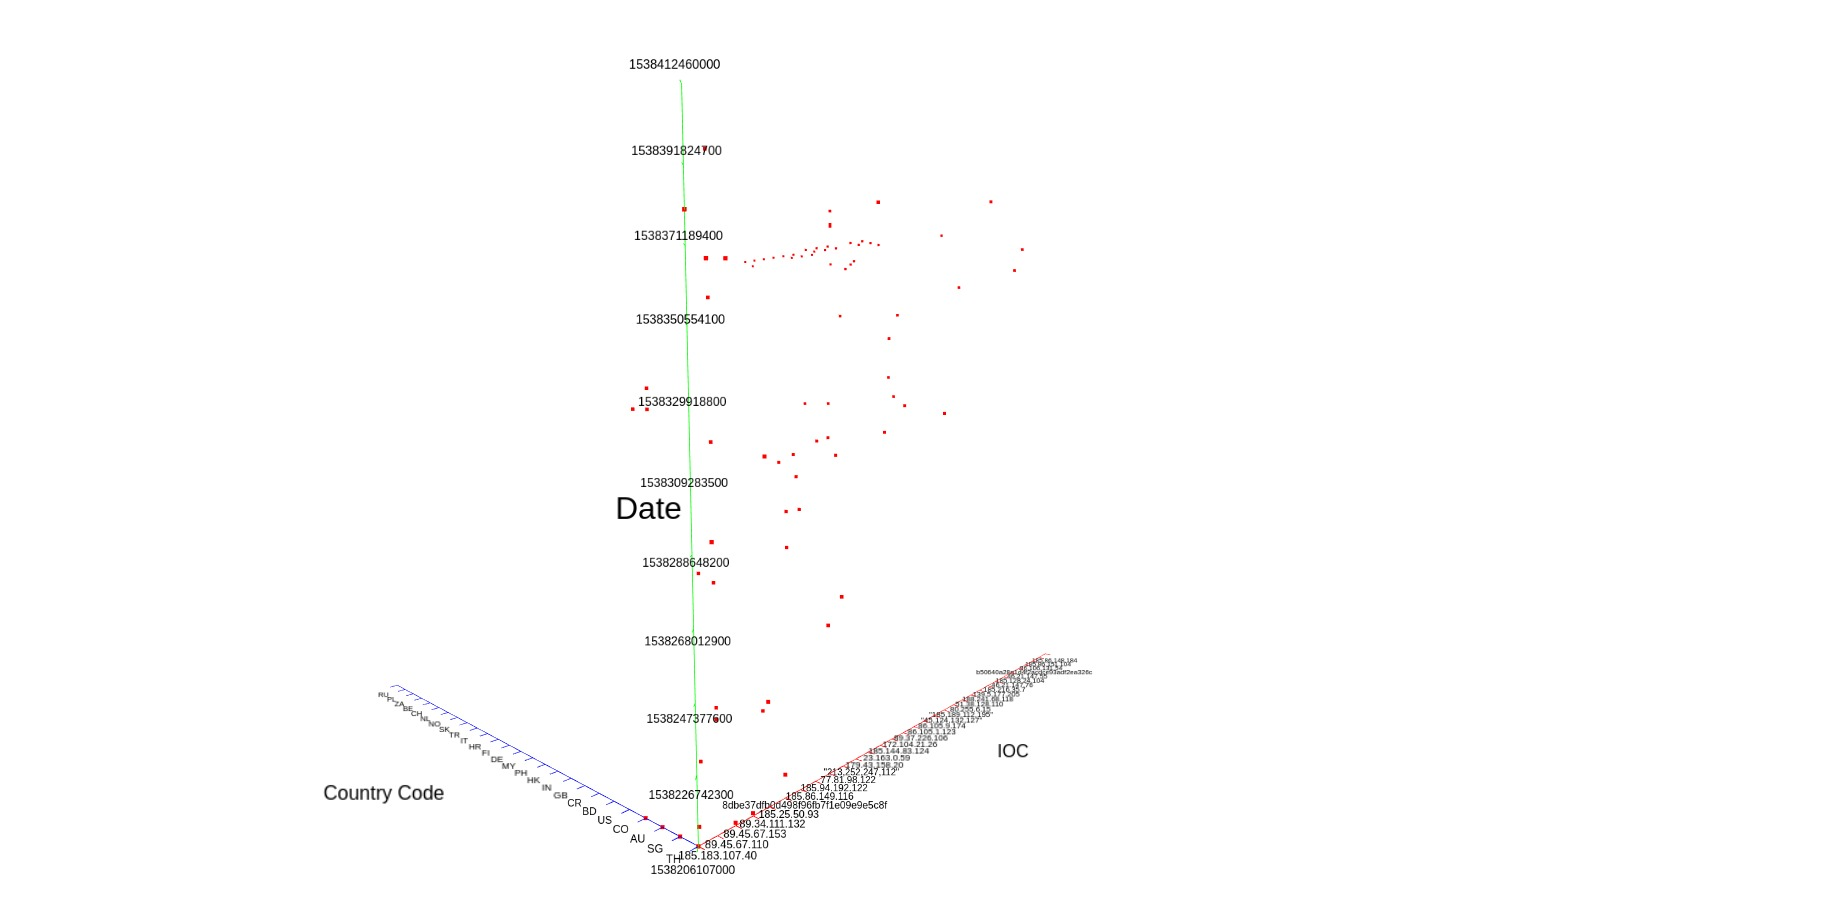
\includegraphics[width=\linewidth]{graphics1.jpeg}
        \caption{Example scatterplot derived from CSV file angled from the outside of the axis}
    \end{figure}
    \begin{figure}[H]
        \centering
        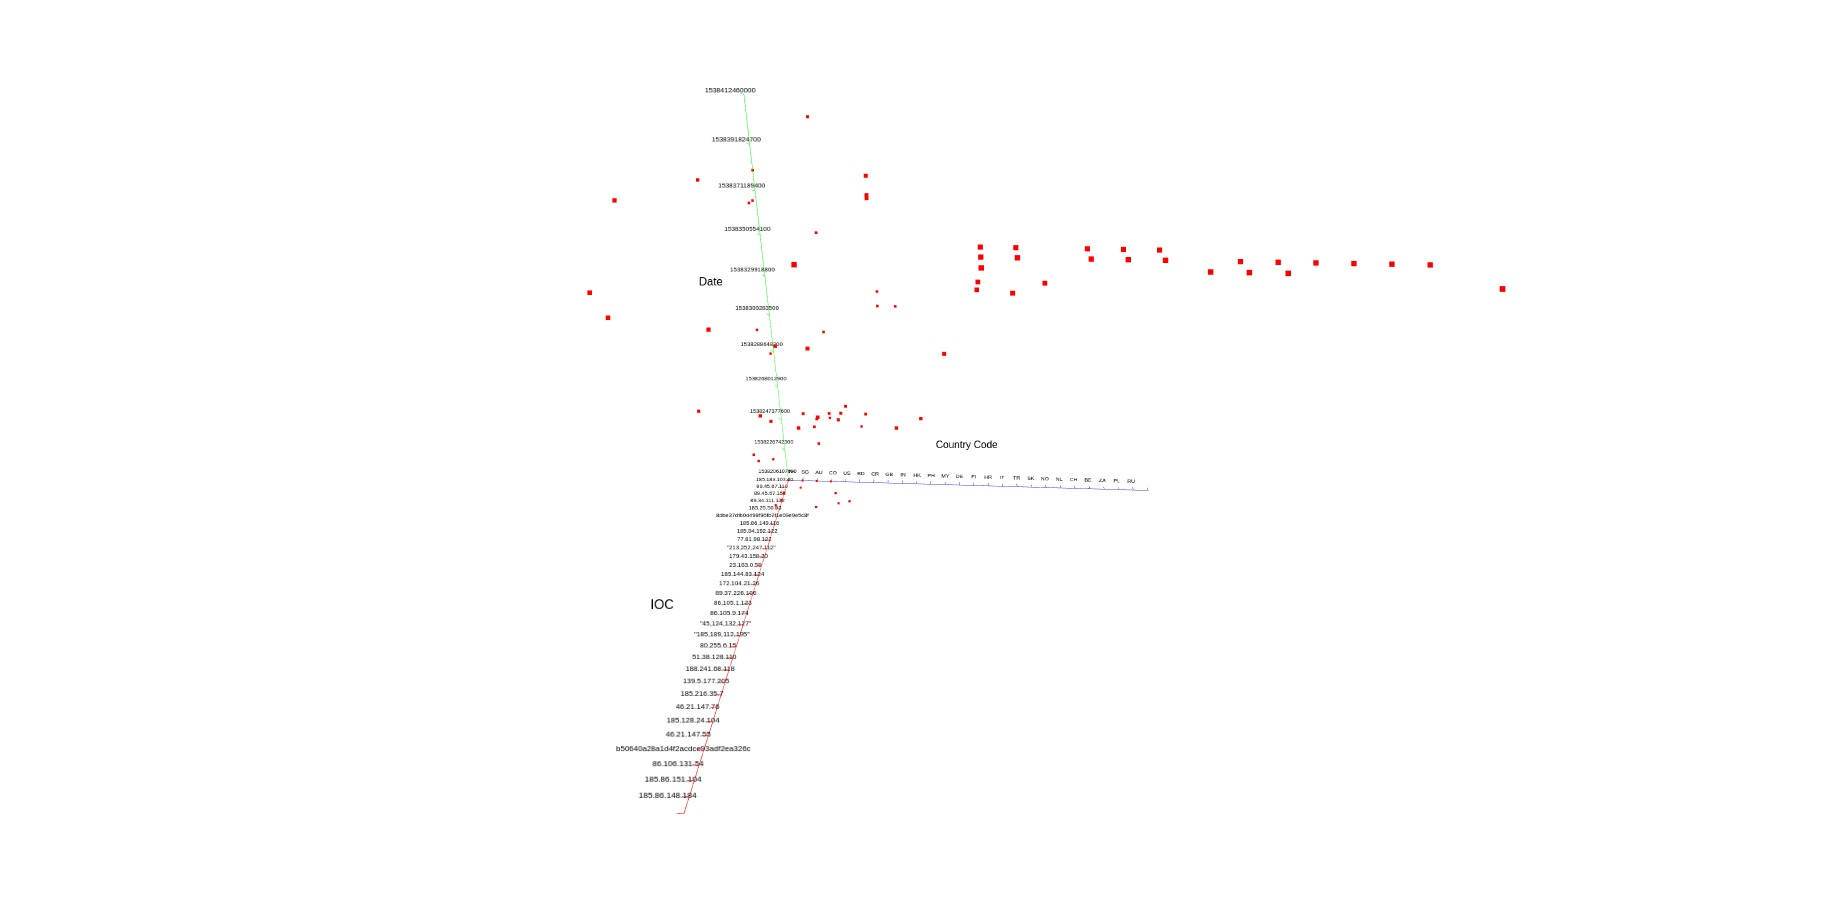
\includegraphics[width=\linewidth]{graphics2.jpeg}
        \caption{Example scatterplot derived from CSV file angled from the inside of the axis}
    \end{figure}
 The above figure will be contained in an interactive environment within the web-page seen in the previous images. If a user wishes to download an image, they can take a screenshot using the \emph{Download} button in the menu. Selecting this button in the menu activates a trigger which takes the current HTML canvas element, converts it into an encoded string, and downloads the string as a \emph{jpeg} image type via the user's browser. 

 \section{Current Issues and Solutions}
 \subsection{3D Visualization}
 As of right now, our biggest issues is that the creation of a new visualization from the given CSV file that could visualize the relationship between the three axes. Currently, we only implement scatter plot and possibly bar chart for next quarter. However, we want something original of our own. We have no solutions for this. Perhaps we have to discuss in the upcoming quarter on how to better visualize the relationship of the given CSV file. Perhaps a line shown between a point or a bar is necessary to better show the relationship between data. The backup solution would be to give this research to the next generation of senior project group. 
 
 \subsection{User Interface}
 The User Interface changed a lot over the whole quarter. We found some issues which we tackled on the way in the term. Since the start of the term the User Interface has changed looks many times. We had a issue at the start which made it such that the User Interface wasn't compatible and wasn't providing enough space for the 3D Visualization, for which we then changed the User Interface that it only had drop down menu instead of having a movable  menu. We even made sure that the web application logo on the top of the page was in such a manner that no hindrance was caused to the 3D Visualization. The other issue was that there were no set of guidelines there on the web application which could probably guide the user to use the web application. To fix that issue we made sure to add a help button which has a set of instructions. We make the User Interface compatible and look in the same style we even made sure that all the buttons were of the same style. The last and the most recent issue which we faced was to make the 3D visualization come to back to its original style from the zoomed in or zoomed out mode. For which there is ongoing development going on and it needs to get client approved.
 
 \subsection{CSV Parsing}
 Throughout the term, CSV parsing has been somewhat trivial, however there were definitely obstacles that proved difficult to find solutions to. One of these issues entailed parsing CSV data that contained commas in the elements - this is due to the fact that some outputs of logging platforms will log IP addresses with commas instead of periods (for example, 1,2,3,4 instead of 1.2.3.4). As a solution, the CSV team was able to find a regular expression online that solved this issue. Right now, our current issues entail designing JavaScript functions to further filter data before it is serialized into a JSON object and sent to the 3D Visualization team, and receiving this filtering information from the UI team. 
 
 \subsection{Exporting}
 Currently, our beta release is able to download an image of the HTML canvas element to the user's browser in \emph{jpeg} format. We currently know how to take several frames of the HTML canvas element and turn it into a GIF or MP4, however we are currently wondering how these frames will be collected. Adding a new modal just to do this would be too much work, however adding an auto-rotate feature at some customized zoom-level might be ideal. This would require research and work by the UI, 3DV, and exporting teams. 
  
 \section{Remaining Work}
 \subsection{3D Visualization}
 The remaining work for the visualization team is to make data with lot of different graph. For example, what we had in mind right now is implementing a bar chart, which will be discussed next quarter. The solution to do this is pretty straightforward such however, it will require the change of User Interface to enable the option for different type of chart. On the other hand, the implementation of a bar chart can be used by grabbing the current X, Y and Z coordinate values given by CSV parser. With the same property as the Axes, which is MeshLines. A bar can be made with different width from the value of X, 0, Z to X, Y, and Z for each data points given.
 \newline The other remaining task would be to make an interact-able data when the cursor points out to the data points. When interacted, the data point will be highlighted or changed in color and the UI will show all the information regarding that specific data points. We currently do not know how to resolve this problem. However, we are planning to use Raytrace, which will throw away a ray from mouse position to the object on the canvas. This will determine what object that the user wants to click. 
 
 \subsection{User Interface}
 Remaining work for as far as the User Interface team is involved  we may need to work on the help button functionality, camera button functionality and filter button functionality. These functionality will need improvements and consistency which matches the styling. The consistency will be required throughout the application. If we get time in the future we will try to make the User Interface more easy for the user. Some functionalities may vary depending on our client as we still needs to get some things approved from him. 
 
 
 \subsection{CSV Parsing}
 Remaining work for the CSV Parsing team involves adding filtering functionalities that can further narrow what a user might be looking for in the data that they provide the application. Once that filtering information is provided by the UI team through an interface - which requires further design requirements - this filtering will be done before any serialization is done. 

 \subsection{Exporting}
 Remaining work for the exporting team involves having functionalities to download GIF and MP4 filetypes. This will entail using external libraries to convert these encoded strings - similar to downloading an image - to other objects. Although we know these external libraries will work in our application, more research needs to be done by the 3D Visualization team in conjunction with the exporting team to obtain some auto-rotating feature in place. 
 

\bibliographystyle{IEEEtran}
\bibliography{IEEEabrv,References.bib}

\end{document}